 \chapter{The Problem of Trust and Centralization}
 \label{cha:trust_and_centralization}
 \section{Why Centralized Control is Undesirable in this Project}
 The reason for building a decentralized application is mainly that users don't have to trust a central authority with their money and their data. Another reason is that users can rely on the integrity of the data provided by the distributed system. In the fully decentralized peer-to-peer model, there is no central point that can be attacked or tampered with. So the end user can be sure that the data they received from one of the nodes of the network is authentic, or at least they can verify this with digital signatures.
 
 However, if there is a central instance that provides the data, as is the case in the current state of the project, users can never be sure that this central source has not been compromised. As of now, the power lies in the hands of the administrators who control what games users can bet on, and also the results of these games. While security precautions have been taken to ensure that not \emph{anyone} can alter game results or manipulate bets, since only the creators of the \texttt{BetManager} contract on the blockchain can call the functions responsible for this, there is still the possibility of the administrators being bribed, or their private keys being stolen. Furthermore, the administrators could take advantage of their power and use their control for personal financial gain, by providing game results they have bet on, etc.
 
 For all these reasons mentioned above, in its current state, the project ultimately defeats the purpose of being provided on a decentralized platform because it still sources crucial data from a central hand. The whole point of blockchain systems is to not have this central point. Systems built based on the traditional model with a central instance have many advantages like better speed, latency and throughput compared to those novel platforms. The factor of having no single controlling instance is essential and must be preserved in order to not defeat the purpose of this project. The target user, which is someone who rejects centralization in favor of decentralized, distributed systems, can not be satisfied with the system as it is. Countermeasures need to be taken and solutions provided to mitigate these issues. This is where so called \emph{Blockchain Oracles} come in.
 \section{The Concept of Blockchain Oracles}
 In order to receive data from the world outside of the Ethereum network, there needs to be a way for smart contracts to be able to interact with regular web servers, for example through APIs that can be queried over regular HTTP or HTTPS. Blockchain applications themselves cannot directly fetch the data they require, like price feeds, weather data, sports game results, election results, etc. A blockchain oracle is basically just a connector that makes this possible. Usually, the oracle itself is also a contract deployed on the blockchain, that can be accessed at its contract address, and queried through specific methods \cite{oraclizedoc}. There are a number of different implementations of such oracles, for various blockchain platforms.
 \begin{table}[ht]
	\centering
	\begin{tabular}{ | l | l | l | l |}
		\hline
		\multicolumn{4}{ | c | }{\textbf{Blockchain Oracle Implementations}} \\ \hline
		\emph{Blockchain Protocol} & \emph{Orisi} & \emph{Town Crier} & \emph{Oraclize} \\ \hline
		\textbf{Bitcoin} & yes & no & yes \\ \hline
		\textbf{Ethereum} & no & yes & yes \\ \hline
		\textbf{Rootstock} & no & no & yes \\ \hline
		\textbf{EOS} & no & no & yes \\ \hline
		\textbf{R3 Corda} & no & no & yes \\ \hline
		\textbf{Hyperledger} & no & no & yes \\ \hline
		\textbf{Fabric} & no & no & yes \\ \hline
	\end{tabular}
	\caption{\label{tab:blockchain-oracles}Blockchain platforms supported by various oracles \cite{zhangtown}\cite{oraclizedoc}\cite{orisiwhitepaper}}
\end{table}
\\
In the table above, it becomes apparent that the most versatile oracle clearly is the \emph{Oraclize} implementation. This service, \emph{Oraclize}, will be used in the cryptocurrency sportsbetting app, because it provides an extensive documentation and a rich interface. 
\section{Existing Solutions}
\subsection{Oraclize}
Oraclize is the leading oracle service in the blockchain space, supporting a variety of platforms, and even non-blockchain applications \cite{oraclizedoc}. It provides a solution which can demonstrate that the data fetched from the third party source, for example over an API request, has not been manipulated. So called \emph{Authenticity Proofs} are used to accomplish this.
\subsection*{Authenticity Proofs}
In order to guarantee data integrity, a document can be requested from a smart contract in addition to the desired third party data, which is a strong cryptographic guarantee providing that the data has not been tampered with. For this, the trust is shifted away from Oraclize, to technology providers or device manufacturers with good reputation and a lot at stake. An example is the \emph{Ledger proof}, which uses the hardware attestation feature provided by BOLOS, to enable code execution on the Ledger platform. BOLOS is a crypto-embedded operating system built for Secure Elements and Secure Enclaves. Ledger, which is a hardware manufacturer for cryptocurrency cold storage, is a device manufacturer with good reputation and a lot at stake. This is one example of how an authenticity proof might be generated. The Oraclize service currently implements three different types of authenticity proofs:
\begin{itemize}
	\item TLSNotary Proof
	\item Android Proof
	\item Ledger Proof
\end{itemize}
\subsection*{TLSNotary Proof}
\emph{TLSNotary} is an open-source protocol and a mechanism for independently audited HTTPS sessions. The technology is developed and used by the \emph{PageSigner} project\cite{pagesigner}. 

It works by splitting the secret data (premaster secret) used to setup the https session to the desired data source, \ie the server, between the auditee (in this case Oraclize) and the auditor (in this case a locked-down AWS instance of an open-source Amazon Machine Image). In this way, it is possible for the auditee, Oraclize, to prove to the auditor that certain web traffic has occurred between them and a server, and that the traffic has come, in fact, from the server (data origin authentication). The server would be the data source requested by the issuer of the "oraclize\textunderscore query" call, such as a machine that serves data over a REST API URL. This authenticity proof is indisputable, provided the auditor trusts the public key of the server (the data source)\cite{tlsnotarywhitepaper}\cite{oraclizedoc}.

The basic steps of how the TLS secret data is split into two parts, and the control flow of how the auditor makes sure that the auditee doesn't produce manipulated data, can be outlined as follows:

\begin{enumerate}
\item Auditee and auditor generate 24 bytes of the premaster secret each, the full premaster secret is not known to either of them.
\item Both, auditee and auditor, apply a hash function to those 24 bytes, generating 48 bytes (auditee $\rightarrow H_1$ and auditor $\rightarrow H_2$).
\item Auditor gives the first half ($H_{21}$) of their hashed secret to auditee.
\item Auditee gives the second half ($H_{12}$) of their hashed secret to auditor.
\item Using these halves, by applying the XOR logical operation, ($H_{11} \oplus H_{21} \rightarrow$ auditee's master secret, and $H_{22} \oplus H_{12} \rightarrow$ auditor's master secret), each party constructs their half of the master secret, which is then further processed to obtain the initialization vectors (IVs), encryption keys, and message authentication codes (MACs) used in the TLS protocol.
\item Both parties compute a hash (140 bytes) of their master secret halves.
\item The auditor gives approximately 120 bytes (exact number depends on the cipher suite) of this hash to the auditee, enabling them to compute IVs, client MAC key, and encryption keys (by XORing the bytes of the hashes). At this point, the client can write the https request and send it to the server. This can be seen as the start of the audit.
\item The server (the desired data source of truth) then responds, the response is received by the client, but not decrypted. Instead, the network traffic is logged, a hash is computed and sent to the auditor (commitment of the auditee). This is the key point in the whole auditing process, as this commitment (the hash), can later be used to prove the authenticity of the data, since there was no way for the client to fabricate fake traffic data using the server mac that they don't have at that point.
\item After the auditor receives this commitment, they reveal the remaining approximately 20 bytes, and send them to the auditee. This allows them to compute the server mac key. The TLS process continues from there, the auditee decrypts the network traffic, and checks authenticity with the server MAC.
\end{enumerate}
The process is illustrated in detail in the following figures:

\begin{figure}[H]
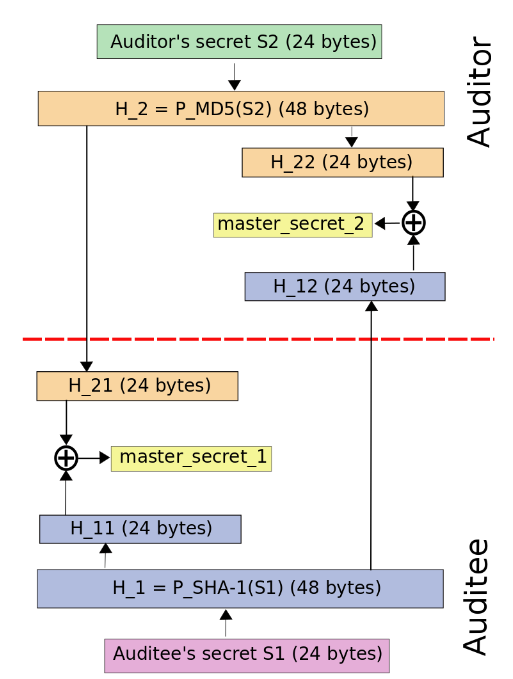
\includegraphics[scale=0.5]{tlsnotary_secret_splitting}
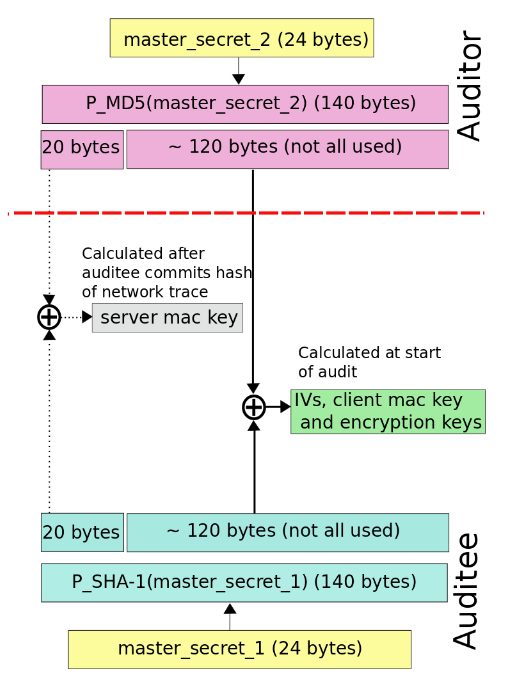
\includegraphics[scale=0.5]{tlsnotary_secret_splitting_2}
\caption{Control flow of the TLS secret splitting and auditing process. \cite{tlsnotarywhitepaper}}
\end{figure}

This series of complex steps is done so that the auditee (Oraclize) cannot create a fake version of the HTTP traffic from the server, since they do not have the server mac key. Only once the auditor releases the remaining 20 bytes of the expanded key block (generated from the master secret key halves), the auditee can complete the TLS decryption and authentication steps, view the data, and forward it to the issuer of the oraclize request. 

In this way, the creator of a smart contract using Oraclize can be sure that the data forwarded by this service has not been tampered with and is authentic.

\newpage

\subsection*{Android Proof}
Android Proof is another type of Oraclize's authenticity proofs. It uses Google's \emph{SafetyNet} Software Attestation and Android Hardware Attestation in order to provide an environment that is secure and auditable, which can deliver reliable data.

The basic concept is to use a service application, which is running on a trusted physical Android device, to fetch and deliver this data. The integrity of this device is guaranteed by \emph{SafetyNet}, which can prove that the list of root certificate authorities stored on the device has not been modified. It does this by verifying the full chain of certificates against publicly available certificate revocation lists owned by Google. \emph{SafetyNet} can also detect whether an Android device is in a tampered state or not.

Another important part of this type of proof is the Hardware Attestation Object, which is required to prove that the key has been generated inside the KeyStore of the trusted physical Android device.

The process of retrieving data from an API while using the Android Proof attestation can be outlined in the following way\cite{androidproof}:
\begin{itemize}
	\item The URL provided by the issuer of the oraclize request (the data source URL) is sent to the trusted Android device. The service application running on this device then establishes a HTTPS connection with this URL, and the entire response is retrieved from the server. Then the SHA256 hash of this response is calculated and signed by the application, using the hardware attested key pair from the Android KeyStore on this device.
	\item A call to Google's SafetyNet API is made using the data from before as parameter. The API returns an \emph{AttestationResponse} in the JSON Web Signature format (JWS).
	\item The service application running on the trusted device then sends the entire JWS response, the HTTPS response with its SHA256 signature and the requestID to Oraclize. There the proof is validated and the data from the HTTPS response is forwarded to the issuer of the oraclize request. The SafetyNet AttestationResponse and the Hardware Attestation Object are also sent to the issuer.
\end{itemize}

The following picture demonstrates this process in a simplified way:
\begin{figure}[H]
\centering
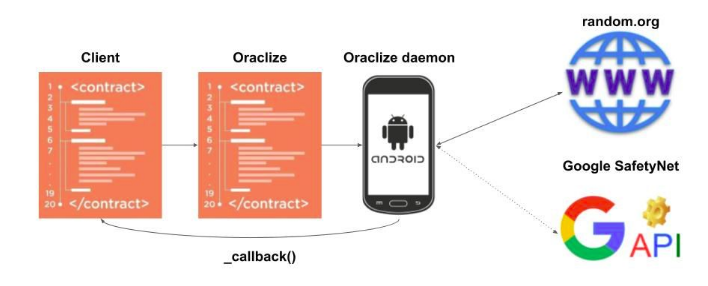
\includegraphics[scale=0.75]{android_proof_process}
\caption{Oraclize API request using Android Proof\cite{androidproof}}
\end{figure}
This type of authenticity proof can be verified by any third party by checking the following elements:
\begin{itemize}
	\item JWS Verification, this can be done by validating the certificate chain found in the JWS Header against a certificate revocation list by a known root certificate authority.
	\item SafetyNet Authenticity. For this, the Google Device Verification API can be consulted to check if the JWS has indeed been generated by Google.
	\item SatetyNet Response Verification
	\item Hardware Attestation Verification
\end{itemize}

In order for the Android Proof to be a suitable method for guaranteeing data authenticity, a number of features of the Android platform are utilized. Worth mentioning here are the Android Hardware Keystore and the Hardware Attestation, first implemented in Android Nougat. Both features are implemented in a TEE (Trusted Execution Environment). Furthermore, the concept relies on Google's SafetyNet Software Attestation APIs and the Android App Sandbox model. It is assumed that this model is secure and prevents apps from manipulating memory or data that do not belong to them. This sandbox model is one of the key features of the Android OS. Google's SafetyNet is a feature which can be used by developers to check whether a device is in a tampered (rooted, monitored, infected with malware) state or not.

The steps of generating this Android Proof are outlined in more detail in the following graph, taken from the Android Proof whitepaper by Oraclize.

\begin{figure}[H]
\centering
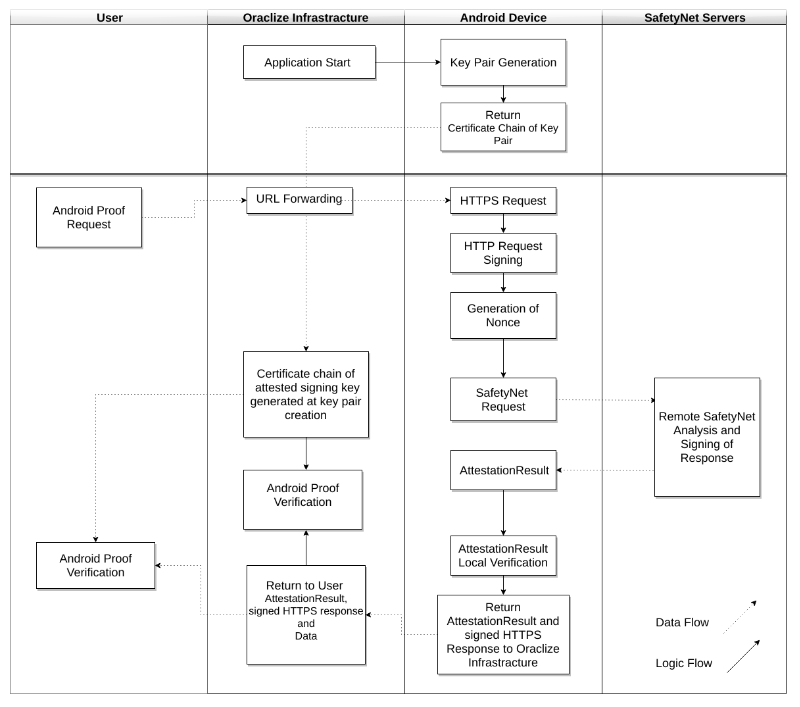
\includegraphics[scale=0.66]{android_proof_detailed_graph}
\caption{A detailed graph showing how the Android Proof is generated and verified\cite{androidproof}}
\end{figure}
\subsection*{Ledger Proof}
The third kind of authenticity proof provided by the Oraclize service is called \emph{Ledger Proof}. \emph{Ledger} is a French company specializing in the field of producing hardware-enforced cryptocurrency wallets. Their flagship product is the Ledger Nano S. Their devices are equipped with a STMicroelectronics secure element, a controller and the operating system \emph{BOLOS}. Developers can build applications for this OS using the BOLOS-SDK.

The feature in the \emph{BOLOS} operating system which is important to Oraclize is the kernel-level API which can conduct cryptographic operations and attestations. The attestation feature enables any application, by querying the appropriate API, to retrieve a signed hash of the kernel binary. This hash is signed using a key which is controlled by the BOLOS kernel and can not be accessed by the application developer. Furthermore, this key has a full chain of trust with the root in a master key that resides on a hardware security module controlled by Ledger.

These features of the BOLOS operating system are utilized by Oraclize to attest to the user of the Oraclize query system that the applications built by Oraclize are indeed running in a trusted execution environment (TEE) of a true Ledger device\cite{oraclizedoc}.


There are tools available to verify the proofs generated by Oraclize \cite{oraclizeproofverify}.
\subsection*{Oraclize Engine}
The basis for the functionality of the Oraclize service is the \emph{Oraclize Engine}. Internally, it replicates a logical, conditional model. Thus, certain conditions can be verified repeatedly and data will only be returned if those conditions are met. In order to form a valid request, the engine needs to be provided with at least two, or optionally three arguments:
\begin{itemize}
	\item A data source type
	\item A query
	\item (Optional) An authenticity proof type
\end{itemize} 
Those arguments are passed as string arguments to the \texttt{oraclize\textunderscore query} function call. An example call could look like this:

\texttt{oraclize\textunderscore query("URL", "xml(https://www.example.at/api).element");}
\subsection*{Data Source Types}
In the example above, the data source type was "URL", however Oraclize supports various other types, such as\cite{oraclizedoc}
\begin{itemize}
	\item WolframAlpha: native access to WolframAlpha engine
	\item IPFS: access to any file stored on IPFS (InterPlanetary File System)
	\item Random: provides random data utilizing the Ledger Authenticity Proof type
	\item Computation: the result of a computation specified by the issuer of the query
\end{itemize}
Furthermore there are meta data source types, including:
\begin{itemize}
	\item Nested: used for nesting multiple data source types of different kind, or multiple requests to one source, returns one unified result
	\item Identity: returns the query
	\item Decrypt: decrypts data which was encrypted with the Oraclize private key
\end{itemize}
\subsection*{Queries}
The query is the central element to be used in the Oraclize engine. It specifies the details of the request containing information where the data is to be retrieved from, for example a specific URL.

On a technical level, the query is an array of parameters, with the first one being mandatory. An example is the URL where a certain resource is located. However, the result of this query may not be suitable in the original format, it may need to be parsed. For this, Oraclize provides parsing helpers, which can be specified within the query.
\subsection*{Query Parsing Helpers}
There are JSON, XML, XHTML and binary parsing helpers offered by the Oraclize service. They are used by prefixing the name of the data format (e.g. "json") to the query and appending object, tag names or operators, depending on the format. An example using a parsing helper for binary data source types could look like this: 

\texttt{binary(http://www.siemens.com/pki/ZZZZZZVS.crl).slice(0,300)}

The parameters of the slice operator are \texttt{(offset, length)}. This example will return the first 300 bytes in this binary file.
\subsection{Verity}
Verity is a platform for decentralized data feeds. It has a conceptually different approach to fetching data, when compared to Oraclize. Instead of connecting to Web-APIs, it sources the data by using wisdom of the crowd and blockchain-as-a-court-system\cite{veritywhitepaper}.

Basically, the core concept of this service is to create an incentive for people to provide truthful data about real-world events. This is done by giving participants monetary rewards, in the form of cryptocurrencies, if they provide correct information about events that have happened in the world.

The correctness of information in this system is determined by a rather complex consensus mechanism. Data providers (mostly people observing real world events) report on events via a desktop or mobile app. They can enter what the values of pre-defined parameters of a data request are, for instance, which team won a football game. The data request is made by developers of smart contracts that rely on data from the outside world, such as the outcome of a sports game, how many yellow cards were raised in a game, how many people attended an event, etc. The basic flow of information from the data providers to the developers is illustrated in the following figure:
\begin{figure}[H]
\centering
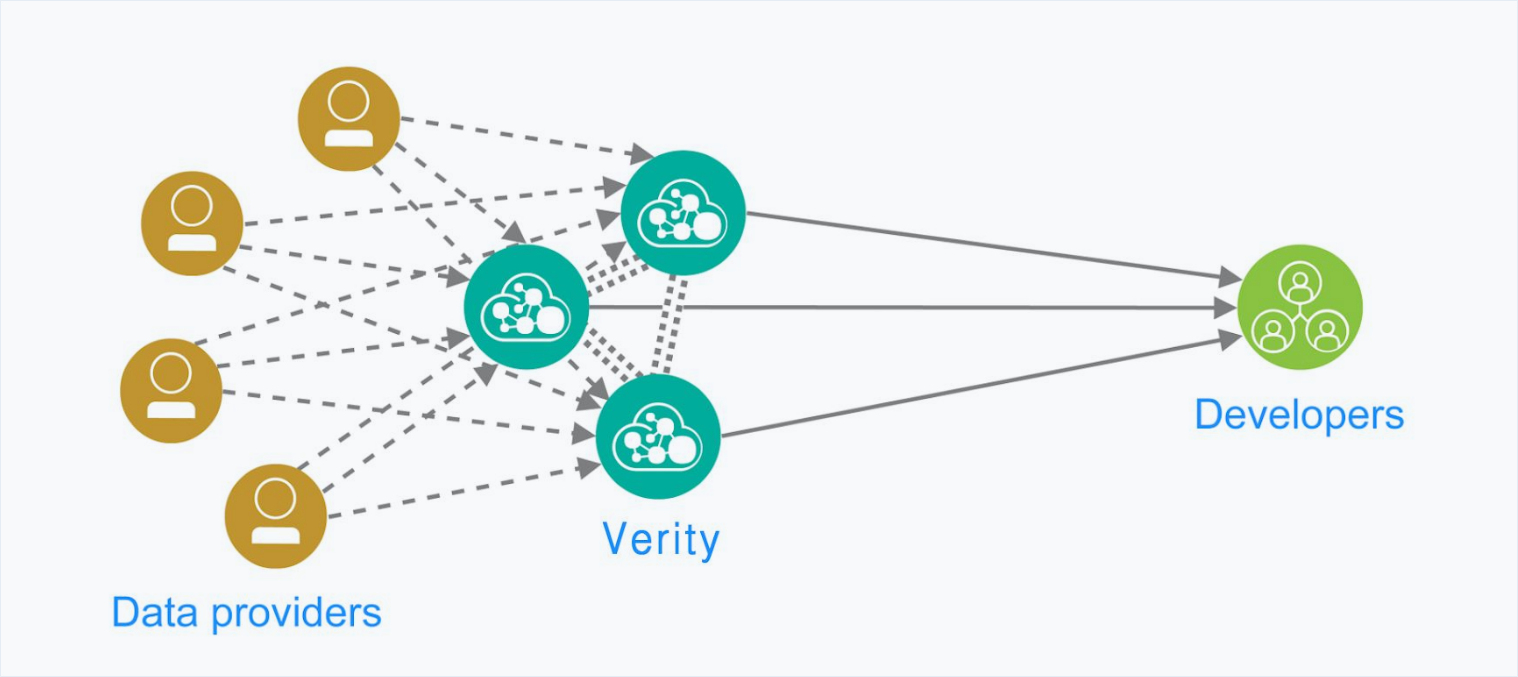
\includegraphics[scale=0.27]{verity-data-flow}
\caption{The flow of information in the verity network\cite{veritywhitepaper}}
\end{figure}

On the left hand side are the people that observe the events, of which the developer (of a smart contract) wants to know the outcomes. In the middle are the Verity network nodes, which validate the data by forming a consensus (\eg a specified percentage of data providers report the same information). The parameters for this consensus, such as percentage of same value reports, minimum number of participants, etc., can be defined by the developer. 

\subsection*{Verity System Architecture}

The architecture of the system is split into three parts, the core layer, the services layer, and the application layer. The core layer implements the consensus mechanism and node communication (discovery, routing, message propagation, \etc) and the services layer implements the Verity API, a data feed engine and a marketplace system. The application layer consists of validation nodes, data providing nodes, and provides a Verity SDK and analytics.

The Ethereum blockchain is used as the base layer for the system, plus \emph{Swarm}, which is a decentralized storage platform and content distribution service\cite{swarm-homepage}.

The following graphic provides a good overview over the architecture of the entire system:
\begin{figure}[H]
\centering
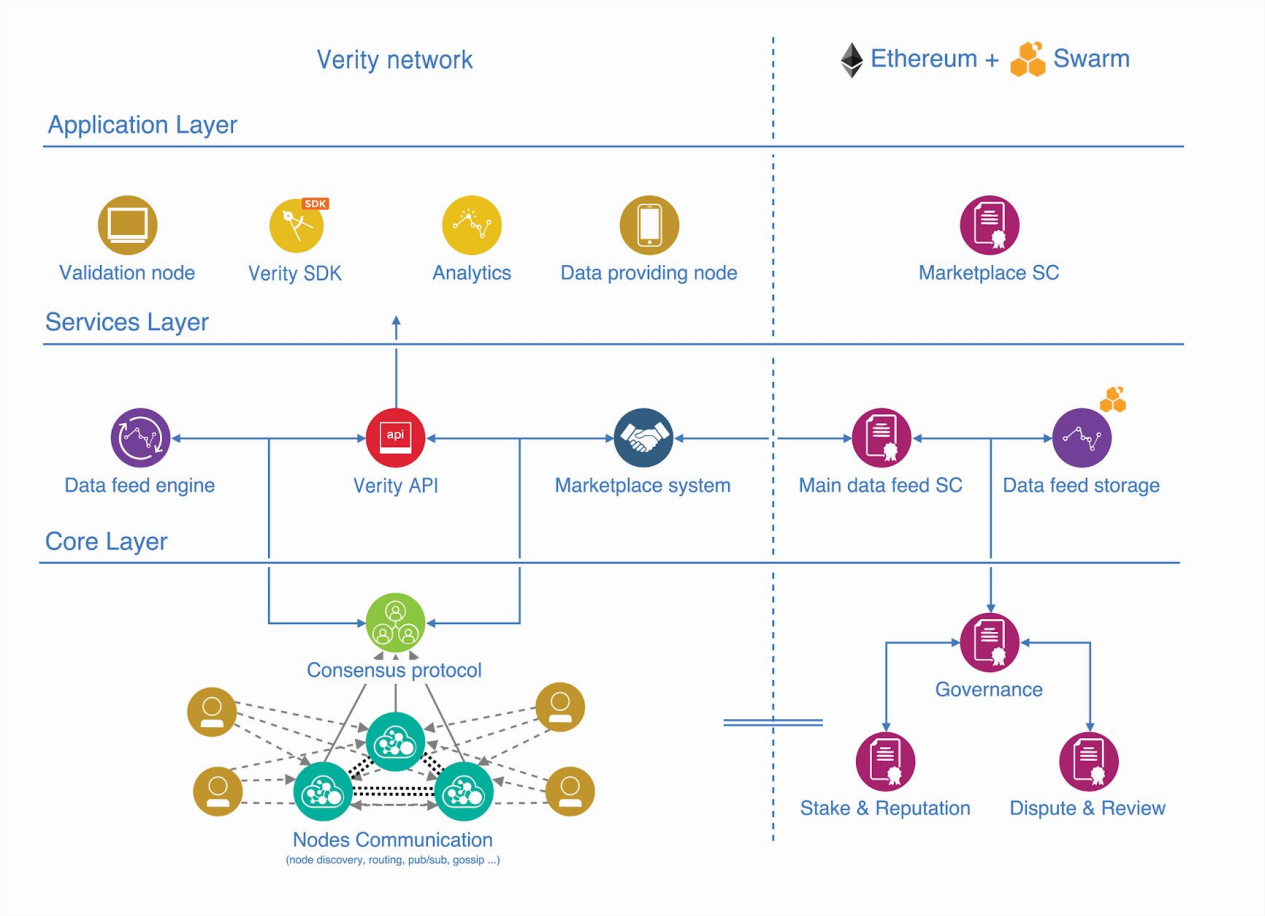
\includegraphics[scale=0.32]{verity-architecture}
\caption{The architecture of the Verity Network\cite{veritywhitepaper}}
\end{figure}

\subsection*{Data Markets}
In order to receive data from the Verity network, a developer first needs to specify what kind of data she wants, in what format the data should be provided, how the consensus for this data should be established, and how much she is willing to pay for this data\cite{veritywhitepaper}. This is necessary to incentivize people to provide high quality, truthful data.

This process is called \emph{market generation}. In Verity, a market can consist of one or more \emph{data feeds}, and each data feed contains at least one or more \emph{data fields}, which represent events, such as whether a penalty kick was successful (boolean), what the end score in a tennis game is (two integers), or even more complex things, like what the name of the current president of a certain country is (string).

The following figure illustrates what a data market in Verity consists of:
\begin{figure}[H]
\centering
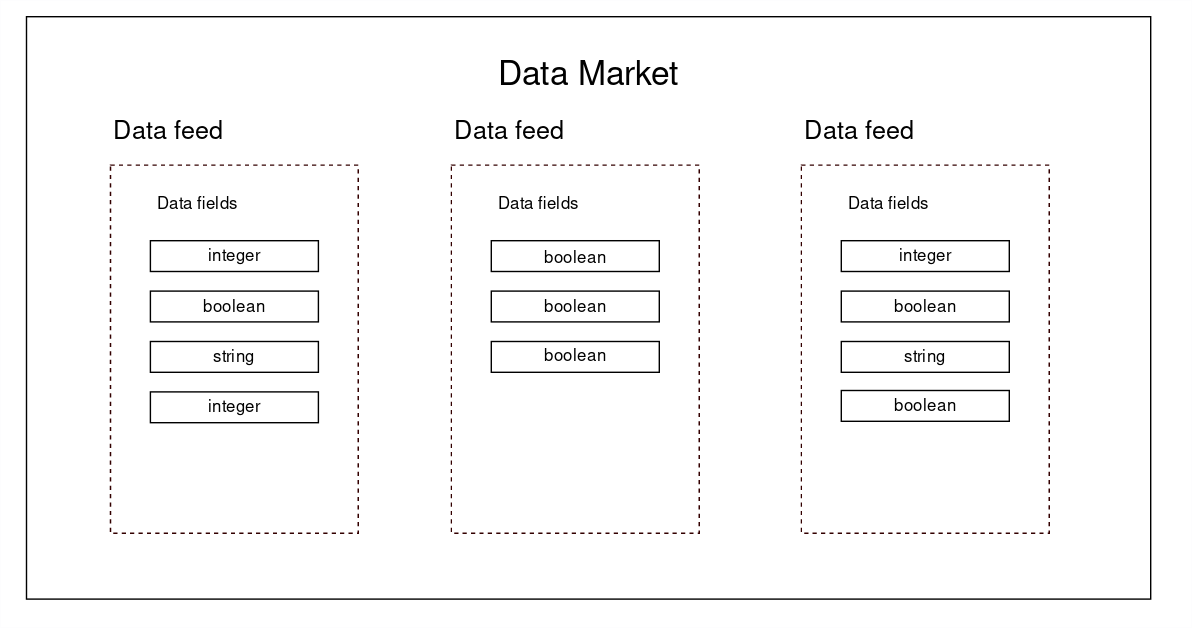
\includegraphics[scale=0.33]{verity-data-market}
\caption{The structure of a data market in Verity}
\end{figure}

Data providers populate this data feed with information. If there are multiple data fields in a data feed, a consensus is only reached, if all of the fields have the same value. 

\subsection*{Verity Network Nodes}
In the Verity network, there are two different kinds of nodes: \emph{Validation} nodes, and \emph{Data Providing} nodes.

\subsection*{Validation Nodes}
Validation nodes capture data, form the consensus according to the rules set by the developer, and send the data to the developer. The also earn fees for correctly processing data (according to the system's rules). Validation nodes are part of a reputation system, and can vote in the governance of the entire system, where each vote is weighted by the node's reputation.

Before a market is created, validation nodes for validating the data in this market are selected randomly. Validation nodes always process \emph{encrypted} data\cite{veritywhitepaper}.

\subsection*{Data Providing Nodes}
Data Providing Nodes do not partake in any consensus forming or voting, they are only there to send data to the validation nodes.

\subsection{Astraea}
Astraea is a decentralized blockchain oracle, described in a paper by John Adler et al.\cite{astraea}, however it has never been implemented as a real world service. Other than Oraclize, it is not an intermediary for fetching data from third party sources, but attempts to deliver data based on a voting game that decides the truth or falsity of propositions.

In the proposed system, there are players (submitters, voters and certifiers) that behave in the following way:
\begin{itemize}
	\item Submitters allocate money to fund propositions that get voted on
	\item Voters submit deposits, and are given the chance to vote on one of the available propositions, chosen at random. The maximum amount a voter can deposit is a parameter of the system.
	\item Certifiers choose an available proposition, and place a large deposit in order to certify its truth or falsity. The minimum deposit for a certification is a system parameter and should be large enough to carry a certain risk.
\end{itemize}
In the paper it is shown that such a system can be set up in a way that manipulation by an adversary is almost impossible, even if the adversary contains up to 25\% of all votes\cite{astraea}.

\subsection{ChainLink}
\emph{ChainLink} is another provider of oracle services in the blockchain space. Currently, the service is available only on the Ethereum test networks, that is Ropsten, Rinkeby and Kovan.

One unique characteristic of \emph{ChainLink} is that the service utilizes the dedicated \emph{LINK} token to carry out transactions. 
\subsection*{Requirements for requesting data}
In order to request data using the ChainLink oracle, some requirements need to be met:
\begin{itemize}
	\item The contract which carries out the request needs to be funded with  LINK tokens. On the test networks, one LINK token amounts to one request.
	\item Depending on the type of data to be requested, a "Job ID" needs to be specified. This is different on every network.
\end{itemize}
For testing purposes, LINK tokens can be obtained from a faucet, which is a contract that gives out free tokens. An example for this is a faucet that runs on the Ropsten testnet, accessible via HTTP at \texttt{https://ropsten.chain.link/}. The address of the contract which calls the request function of the ChainLink contract is entered into the input field on this website, in order to receive LINK tokens.

The "Job ID" for each type of data is found in the ChainLink documentation: \texttt{https://docs.chain.link/docs/addresses-and-job-specs}. For instance, if the contract owner wants to request boolean data, the corresponding "Job ID" would be
 
\texttt{7ac0b3beac2c448cb2f6b2840d61d31f}. It is advisable to store those jobs ids in a constant in the contract, like this:

\begin{SolidityCode}
bytes32 constant UINT256_MUL_JOB = bytes32("493610cff14346f786f88ed791ab7704");
\end{SolidityCode}

To specify HTTP POST or GET parameters, or to navigate through a JSON object, methods within \texttt{Chainlink.Request} can be used. For example, to fetch the current Ethereum USD price over an API, the function can look as follows:
\begin{SolidityCode}
function requestPrice(string _currency) public returns (bytes32 requestId) {
	Chainlink.Request memory req =
	newRequest(UINT256_MUL_JOB, this, this.fulfillEthereumPrice.selector);
	req.add('get', 'https://some-crypto-api.com/data/eth');
	req.add('path', _currency);
	requestId = chainlinkRequest(req, 1 * LINK);
}
\end{SolidityCode}

\subsection*{Receiving data}
In the \texttt{requestPrice} function implemented previously, a callback function that has been assigned to \texttt{requestId} is returned. This function is triggered, when the Chainlink network responds to the query with a result. 
\subsection*{External Adapters}
Chainlink provides a feature called "External Adapters". Basically, these adapters represent the bridge between the Chainlink node, which handles, amongst other things, signing transactions for the blockchain and writing to the blockchain, and complex external APIs that may require some form of authentication.

Publicly open APIs can be read by the Chainlink node directly, without any adapters. However, some APIs require authentication with sensitive credentials. These should not be stored on the Chainlink node directly, as that would pose a security risk. Credentials can be stored in whatever way it is specified in the external adapter.

Furthermore, these adapters can include additional functionality. They can be written in any language\cite{chainlinkdoc}.

\newpage

\subsection*{Architecture Overview}
The Chainlink system architecture is outlined in a simplified way in the following figure:
\begin{figure}[H]
\centering
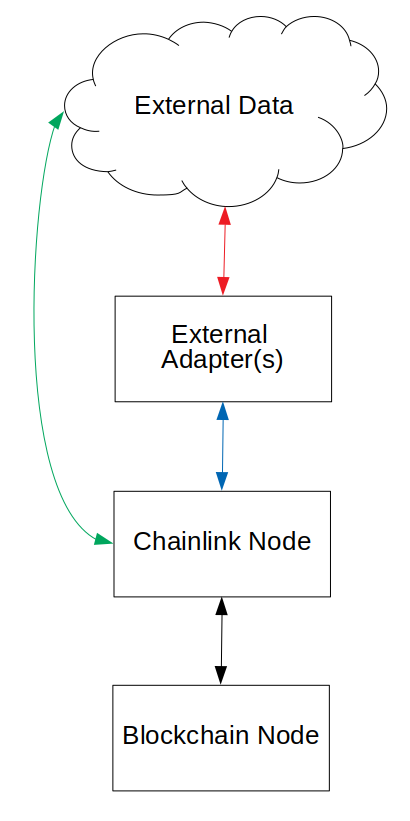
\includegraphics[scale=0.4]{chainlink_architecture}
\caption{The ChainLink system architecture, as described in the official documentation\cite{chainlinkdoc}}
\end{figure}

\section{Implementation of an Oracle in an App}
In the following section, the implementation of an Oracle in an App is demonstrated using the \emph{Oraclize} service. The first steps of extending an app to work with Oraclize, is to fetch the connector contract from Github. It can be found under this URL: \texttt{https://github.com/oraclize/ethereum-api/blob/master
\\
/oraclizeAPI\textunderscore 0.5.sol}. This source code needs to be downloaded and saved into the \texttt{/contracts} directory. The name should be \texttt{usingOraclize.sol}. This contract contains the main logic and the adapters for communicating with the external APIs.

For simulating a blockchain environment, the \emph{Ganache} application is used, as mentioned in chapter \ref{cha:theapp}. The local blockchain will be served from the host \\
\texttt{http://192.168.0.108:7545}, although that URL can be changed in the application settings. When first launching the application, no transactions will be visible in the "Transactions" tab, as seen in the following figure:
\begin{figure}[H]
\centering
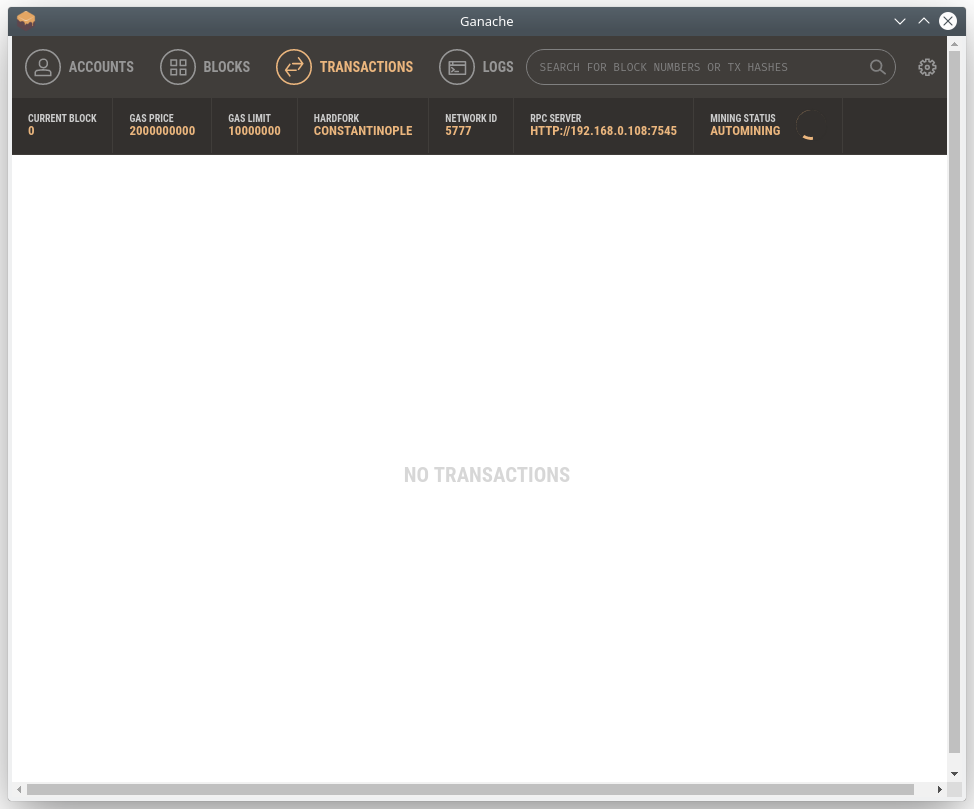
\includegraphics[scale=0.4]{ganache_no_transactions}
\caption{The Ganache application at first startup. The list of transactions is empty.}
\end{figure}
The next step is to compile all of the smart contracts, and deploy them to this local blockchain using the migration script \texttt{1\textunderscore initial\textunderscore migrations.js}. After that the second migration script \texttt{2\textunderscore deploy\textunderscore contracts} is run. These processes can be automated by simply running the command \texttt{migrate --reset} in the \emph{truffle console}. 
\begin{GenericCode}[numbers=none]
truffle(development)> migrate --reset
\end{GenericCode}
After successfully completing, a summary of the deployment costs is displayed on the console:
\begin{GenericCode}[numbers=none]
	> gas used:				5423581
	> gas price:			20 gwei
	> value sent:			0 ETH
	> total cost:			0.10847162 ETH
	
	
	
	> Saving migration to chain.
	> Saving artifacts
	----------------------------------
	> Total cost:			0.10847162 ETH
	
	
Summary
=======
> Total deployments:	2
> Final cost:					0.11525048 ETH

truffle(development)> 
\end{GenericCode}
This console is provided by the \emph{Truffle Suite} software. It greatly speeds up the development, and especially the debugging process of Smart Contract applications. As one can see now, the transactions that have been sent to the local blockchain by the \texttt{migrate --reset} command appear in the "Transactions" tab of the Ganache application.
\begin{figure}[H]
\centering
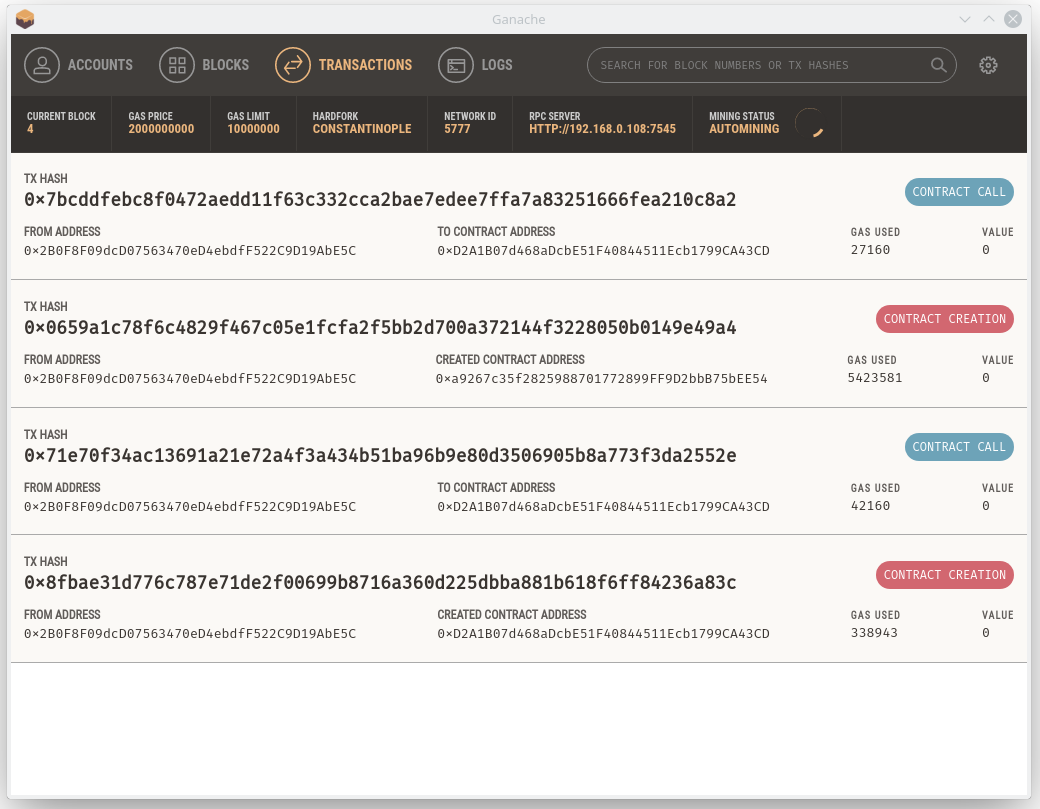
\includegraphics[scale=0.4]{ganache_initial_transactions}
\end{figure}
Now the application lives on this local blockchain. However, there is still no connection to the Oracle, because the \emph{Oraclize} service requires an additional component, the \emph{Ethereum Bridge}, in order to function correctly. The source for this bridge can be obtained from Github: \texttt{https://github.com/oraclize/ethereum-bridge}. The bridge is run by issuing the command \texttt{ethereum-bridge -H 192.168.0.108:7545 -a 9 --dev} in the terminal, in the root folder of the ethereum-bridge. The parameters in this command can be described as follows:
\begin{itemize}
	\item -H specifies the host on which the local blockchain is served
	\item -a specifies which account to use (in this case the 9th account)
	\item --dev specifies that development mode should be used
\end{itemize}
The Ethereum bridge deploys some contracts onto the local blockchain:
\begin{figure}[H]
\centering
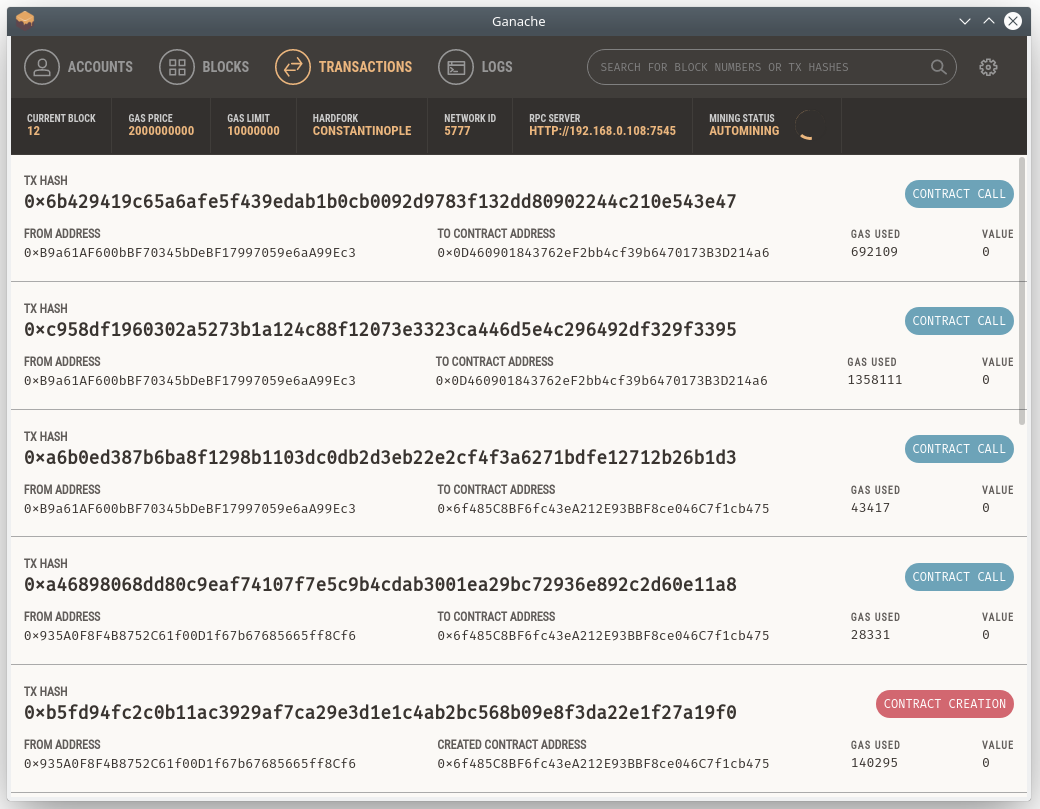
\includegraphics[scale=0.4]{ganache_ethereum_bridge_transactions}
\caption{The transactions generated by the Ethereum list can be viewed in this list}
\end{figure}
Then the Oraclize address resolver is provided by the bridge and needs to be inserted into the constructor of the \texttt{OracleObserver} contract:
\begin{figure}[H]
\centering
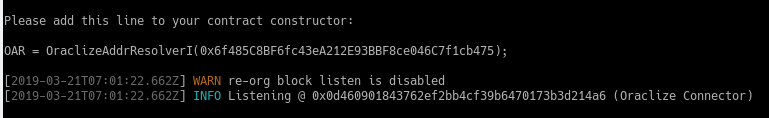
\includegraphics[scale=0.7]{ethereum_bridge_oar}
\caption{The Oraclize address resolver from this terminal output needs to be added to the constructor}
\end{figure}
After that, the setup is completed so far - the Smart Contract can now communicate with the Oraclize service, if the methods are implemented correctly in a contract that inherits from the connector contract. In this project application, that contract is the \texttt{OracleObserver} contract. The crucial functions that are responsible for actually fetching the data, and storing it in a variable in the contract are these following two:

\begin{SolidityCode}
function __callback(bytes32 queryId, string memory result) public {
	if (msg.sender != oraclize_cbAddress())
		revert();
	emit newDataResult(result);
}

function update() public payable {
	emit newOraclizeQuery("Oraclize query was sent, standing by for the answer..");
	oraclize_query("URL", "xml(https://www.datasource.com/ws/rest/gameresults).game.home");
}
\end{SolidityCode}
\captionof{lstlisting}{The implementation of the crucial connector functions in the OracleObserver contract}

After these steps, the data can be successfully fetched from the web API, via these connector functions, and stored in a variable residing in the smart contract. Lastly, there needs to be an interface between the frontend (the GUI presented to the user in the browser), and the backend (the application logic that resides in the contracts and the script functions on the server). This is enabled by the \emph{MetaMask} plugin, which manages the Ethereum accounts, and injects them into the web application through the \emph{web3} library. 
